\documentclass[11pt,a4paper,twocolumn]{article}

% === Core Packages ===
\usepackage[margin=2cm]{geometry}
\usepackage[utf8]{inputenc}
\usepackage[T1]{fontenc}
\usepackage{times}
\usepackage{amsmath,amssymb}
\usepackage{graphicx}
\usepackage{booktabs}
\usepackage{float}
\usepackage{enumitem}
\usepackage{tikz}
\usepackage{pgfplots}
\pgfplotsset{compat=1.18}
\usetikzlibrary{arrows.meta,shapes.geometric,positioning,calc,decorations.markings,fit,backgrounds}

% === Citation (IEEE style) ===
\usepackage[numbers,sort&compress]{natbib}
\bibliographystyle{IEEEtranN}

% === Hyperref ===
\usepackage[hidelinks]{hyperref}
\usepackage{xurl}

% === Settings ===
\setlength{\parindent}{1em}
\setlength{\parskip}{0.3em}

% === Title ===
\title{\textbf{Jaringan Reputasi Terdesentralisasi:\\Kerangka Kerja untuk Organisasi Sosial Alami}}
\author{Pavel Kudrna\\Prague, Czechia\\Draft v1 --- March 2026}
\date{}

\begin{document}
\maketitle

% ============================================================
% ABSTRACT
% ============================================================
\begin{abstract}
Rasa keadilan---keyakinan bahwa kesalahan diperbaiki dan jasa dihargai---adalah kekuatan kohesif terkuat dalam masyarakat. Ketika institusi tata kelola yang tersentralisasi tidak dapat memberikan rasa ini karena biaya menegakkan suatu hak melebihi nilai hak itu sendiri, kohesi sosial pun terkikis. Struktur institusional saat ini gagal menyelesaikan sekelompok besar sengketa dengan cara yang secara sistematis sama seperti perencanaan terpusat gagal mengalokasikan sumber daya: melalui asimetri informasi, hilangnya lingkaran umpan balik, dan terputusnya pengambil keputusan dari konsekuensi keputusan mereka. Makalah ini menyajikan Reputation Social Network (RSN): sebuah lapisan komunikasi yang terdesentralisasi, tidak dapat dikorupsi, dan tahan sensor yang dibangun di atas Decentralized Identifiers (DIDs) yang memungkinkan peserta pseudonim untuk memublikasikan, memverifikasi, dan mengonsumsi informasi reputasi tentang perilaku di dunia nyata. Mekanisme inti bertumpu pada tiga prinsip desain: (1)~struktur biaya asimetris di mana membaca data reputasi itu murah tetapi menulis memerlukan upaya yang dapat diverifikasi; (2)~protokol pemilihan verifikator nondeterministik berbasis consistent hashing yang menetapkan harga bagi klaim radikal melalui biaya iterasi yang meningkat; dan (3)~model otoritas reputasi berbasis pasar di mana verifikator swasta mempertaruhkan reputasi yang telah mereka kumpulkan atas keakuratan klaim yang mereka dukung. Arsitektur yang dihasilkan menghasilkan meritokrasi yang muncul secara emergen tanpa koordinasi terpusat dan memungkinkan jalur migrasi yang bertahap dan dapat dibalik dari sistem yang saat ini dikelola negara.
\end{abstract}

% ============================================================
% 1. INTRODUCTION
% ============================================================
\section{Pendahuluan}

\subsection{Masalah Kepercayaan Tersentralisasi}

Tata kelola modern bertumpu pada asumsi fundamental: bahwa institusi tersentralisasi dapat memediasi kepercayaan antara orang asing dalam skala besar. Pengadilan mengadili sengketa. Registri menyertifikasi kepemilikan. Badan regulasi menegakkan standar. Institusi-institusi ini dirancang pada era ketika informasi langka, komunikasi lambat, dan pendelegasian wewenang kepada badan pusat adalah satu-satunya mekanisme koordinasi yang layak. Namun, tata kelola tersentralisasi gagal karena alasan struktural yang sama seperti perencanaan terpusat: asimetri informasi, hilangnya lingkaran umpan balik, dan terputusnya pengambil keputusan dari konsekuensi keputusan mereka.

Asumsi ini gagal, misalnya, ketika biaya mediasi institusional melebihi nilai sengketa. Bayangkan seorang penyewa yang menemukan bahwa apartemen sewaannya tidak memiliki sertifikat keselamatan listrik yang diwajibkan hukum---suatu kondisi yang menimbulkan bahaya langsung bagi nyawa. Hak hukum penyewa untuk membatalkan kontrak sudah jelas tanpa keraguan. Namun biaya menegakkan hak tersebut melalui sistem pengadilan melebihi nilai moneter dari deposit dan ganti rugi yang terutang, bahkan termasuk potensi kompensasi menurut undang-undang~\cite{czcourtfees}. Respons yang rasional adalah menanggung kerugian dan pergi.

Ini bukanlah kasus tepi yang patologis. Ini adalah pengalaman default untuk sekelompok besar sengketa di mana kerugiannya nyata tetapi taruhan moneternya berada di bawah ambang batas di mana penegakan institusional menjadi rasional secara ekonomi. Hasilnya adalah sebuah sistem yang secara struktural menguntungkan pelaku jahat: mereka yang merugikan orang lain dalam volume di bawah ambang batas ini dapat bertindak tanpa hukuman, karena biaya mencari keadilan jatuh pada pihak yang dirugikan.

Contoh di atas diambil dari lingkungan hukum penulis---sistem hukum perdata Ceko. Dalam tradisi hukum lain---common law berbasis preseden, hukum adat, sistem campuran---keadilan gagal dengan cara yang berbeda dan pada tingkat yang berbeda, tergantung pada kekhususan budaya dan prosedural yurisdiksi tersebut. Pembaca kemungkinan akan mengenali contoh serupa dari konteks mereka sendiri. Yang bersifat universal secara struktural adalah polanya: sengketa yang nilainya jatuh di bawah ambang batas penegakan yang rasional secara ekonomi berakhir dengan kerugian yang ditanggung oleh pihak yang dirugikan. RSN tidak menjanjikan keadilan yang sempurna---ia hanya mengurangi keunggulan struktural yang dinikmati pelaku jahat ketika penegakan institusional tidak ekonomis.

\subsection{Mengapa Solusi yang Ada Belum Memadai}

\textbf{Kerangka Decentralized Identity (DID)}~\cite{did2022} menyediakan mekanisme kriptografis untuk manajemen identitas berdaulat-sendiri tetapi berfokus terutama pada verifikasi identitas tanpa membahas pertanyaan yang lebih luas tentang reputasi perilaku.

\textbf{Soulbound Tokens (SBTs)}~\cite{weyl2022} menangkap wawasan bahwa reputasi tidak dapat dipindahtangankan tetapi bergantung pada infrastruktur blockchain dengan keterbatasan skalabilitas dan tidak membahas insentif ekonomi yang mengatur pemasukan informasi. Konsep terkait seperti merit token (mis., Liberland) memiliki filosofi serupa tetapi tetap terikat pada kerangka yurisdiksi tertentu.

\textbf{Decentralized Autonomous Organizations (DAOs)}~\cite{buterin2014} menerapkan tata kelola melalui smart contract tetapi mereplikasi dinamika plutokratik di mana pengaruh sebanding dengan modal. Quadratic voting~\cite{buterin2019} sebagian mengurangi hal ini tetapi membatasi adopsi praktis. DAO juga menghadapi \emph{masalah oracle} yang fundamental: smart contract tidak dapat memverifikasi keadaan dunia nyata secara andal tanpa sumber eksternal yang tepercaya, dan masalah ini tidak memiliki solusi umum dalam arsitektur blockchain.

Tidak ada sistem yang ada yang menggabungkan desentralisasi, ketahanan terhadap sensor, pseudonimitas, biaya masuk yang dapat diverifikasi, dan konsensus yang emergen.

\subsection{Kontribusi}

Makalah ini memberikan kontribusi sebagai berikut:
\begin{enumerate}[nosep]
\item Definisi \textbf{Reputation Social Network (RSN)}, sebuah protokol terdesentralisasi yang memperluas kerangka DID untuk mendukung pertukaran reputasi bilateral.
\item Sebuah \textbf{protokol pemilihan verifikator nondeterministik} berbasis consistent hashing~\cite{karger1997}.
\item \textbf{Prinsip Radikalisme yang Mahal}, yang menetapkan harga klaim menurut jaraknya dari konsensus jaringan melalui tiga saluran biaya yang bergabung.
\item Sebuah \textbf{model Otoritas Bereputasi} dengan insentif asimetris di mana dukungan palsu berbiaya jauh lebih besar secara katastrofik daripada biaya yang sah.
\item Sebuah \textbf{jalur migrasi bertahap} melalui infrastruktur fiskal paralel.
\end{enumerate}

% ============================================================
% 2. DESIGN PRINCIPLES
% ============================================================
\section{Prinsip Desain}

Arsitektur RSN dibatasi oleh lima prinsip desain yang tidak dapat ditawar.

\textbf{Kontinuitas dan Evolusi.} Sistem ini berdampingan dengan institusi yang ada selama periode transisi dengan durasi yang tidak ditentukan. Transisi tersebut harus dapat dibalik pada setiap tahap.

\textbf{Kesukarelaan dan Tanggung Jawab.} Partisipasi bersifat sukarela, tetapi kesukarelaan dipadukan dengan tanggung jawab: seorang peserta yang mengambil kendali atas suatu fungsi institusional secara bersamaan mengambil kewajiban yang menyertainya.

\textbf{Keberagaman dan Netralitas Budaya.} Konsensus muncul dari interaksi bilateral, bukan dari aturan yang ditetapkan sebelumnya yang dipaksakan oleh perancang sistem.

\textbf{Ketahanan dan Ketahanan terhadap Sensor.} Biaya menyensor jaringan harus melebihi biaya menoleransinya. Hanya totalitarianisme penuh---dengan biaya politik dan ekonomi yang menghancurkan---yang dapat menekan sistem ini.

\textbf{Konsensus dan Penegakan.} Sistem ini menyertakan kecenderungan manusia terhadap kepicikan, kedengkian, dan kepuasan pembalasan sebagai fitur penopang beban. Pelanggaran tidak dilarang; ia diberi harga.

% ============================================================
% 3. SYSTEM OVERVIEW
% ============================================================
\section{Gambaran Umum Sistem}

\subsection{Reputation Social Network}

RSN adalah lapisan komunikasi peer-to-peer yang terdesentralisasi di mana peserta bertukar informasi yang dapat diverifikasi tentang perilaku di dunia nyata. Sifat-sifat yang mendefinisikannya adalah: infrastruktur yang terdesentralisasi dan tidak dapat disensor; partisipasi pseudonim melalui DID; struktur biaya asimetris (membaca murah, menulis mahal); keterverifikasian kriptografis; dan \textbf{dukungan standar}---format yang dapat dibaca mesin untuk informasi yang disebarkan melalui jaringan, untuk layanan yang ditawarkan oleh otoritas (penyusunan klaim, dukungan, layanan saksi), dan untuk format kebijakan termasuk aturan untuk mengevaluasi reputasi pihak lawan serta menilai risiko ketidaksesuaian kebijakan (antara perilaku yang dinyatakan dan yang sebenarnya).

\subsection{Komponen Arsitektural}

RSN terdiri dari empat komponen utama (Gbr.~\ref{fig:architecture}):
\begin{enumerate}[nosep]
\item \textbf{Lapisan DID.} Identitas peserta dengan aturan yang dinyatakan, metadata reputasi, dan perutean jaringan.
\item \textbf{Protokol Klaim.} Format terstruktur untuk memublikasikan pernyataan tentang peristiwa dunia nyata.
\item \textbf{Jaringan Verifikasi.} Protokol terdesentralisasi untuk menugaskan verifikator menggunakan consistent hashing.
\item \textbf{Lapisan Agregasi Reputasi.} Layanan yang menghasilkan ringkasan reputasi yang dapat dibaca manusia.
\end{enumerate}

\begin{figure}[ht]
\centering
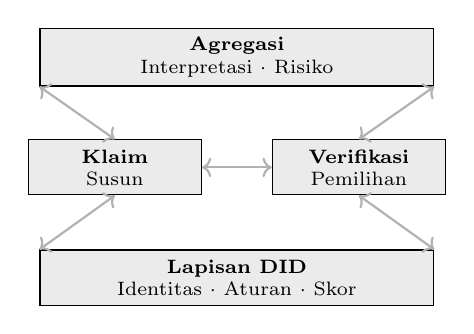
\begin{tikzpicture}[
    layer/.style={draw, minimum height=0.7cm, align=center, font=\scriptsize, fill=black!8},
    arr/.style={<->, thick, gray!60}
]
\node[layer, minimum width=5cm] (agg) at (0,2.8) {\textbf{Agregasi}\\Interpretasi\ $\cdot$ Risiko};
\node[layer, minimum width=2.2cm] (claim) at (-1.55,1.4) {\textbf{Klaim}\\Susun};
\node[layer, minimum width=2.2cm] (verif) at (1.55,1.4) {\textbf{Verifikasi}\\Pemilihan};
\node[layer, minimum width=5cm] (did) at (0,0) {\textbf{Lapisan DID}\\Identitas $\cdot$ Aturan $\cdot$ Skor};

\draw[arr] (agg.south west) -- (claim.north);
\draw[arr] (agg.south east) -- (verif.north);
\draw[arr] (claim.east) -- (verif.west);
\draw[arr] (claim.south) -- (did.north west);
\draw[arr] (verif.south) -- (did.north east);
\end{tikzpicture}
\caption{Arsitektur empat lapisan RSN.}
\label{fig:architecture}
\end{figure}

\subsection{Peran Peserta}

Sebuah transaksi verifikasi melibatkan hingga enam peran DID yang berbeda (Gbr.~\ref{fig:roles}): \textbf{Penerbit} ($DID_I$, membuat dan mengajukan klaim), \textbf{Subjek} ($DID_S$, DID yang menjadi objek klaim---dapat bertepatan dengan Penerbit), \textbf{Otoritas} ($DID_A$, mendukung klaim dengan imbalan; juga dapat menawarkan layanan saksi---\emph{opsional}), \textbf{Saksi} ($DID_{W_{1..n}}$, pemantau kejujuran verifikator secara inkognito melalui kode tantangan---\emph{opsional}), \textbf{Verifikator} ($DID_V$, dipilih secara algoritmik untuk memublikasikan klaim), dan \textbf{RSN} (jaringan tempat klaim yang terverifikasi dipublikasikan). Peran apa pun dapat didelegasikan ke DID lain (Bagian~7.4). Sebuah Otoritas umumnya menggabungkan dukungan dengan layanan saksi, tetapi kedua fungsi tersebut secara logis independen.

\begin{figure}[ht]
\centering
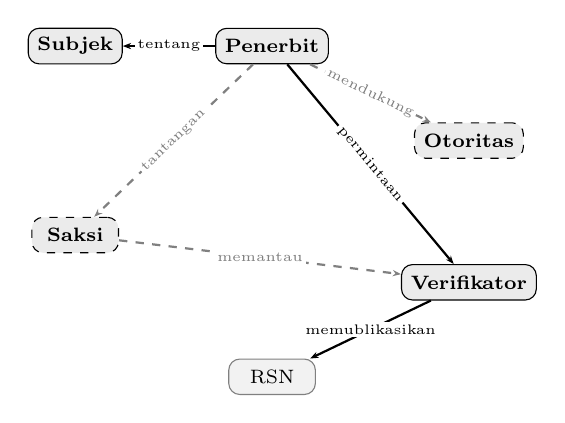
\begin{tikzpicture}[
    role/.style={draw, rounded corners, minimum width=1.1cm, minimum height=0.45cm, align=center, font=\scriptsize, fill=black!8},
    opt/.style={draw, rounded corners, minimum width=1.1cm, minimum height=0.45cm, align=center, font=\scriptsize, fill=black!8, dashed},
    arr/.style={-{Stealth[length=3pt]}, thick},
    oarr/.style={-{Stealth[length=3pt]}, thick, dashed, gray},
    lbl/.style={font=\tiny, fill=white, inner sep=1pt}
]
\node[role] (I) at (0,2.4) {\textbf{Penerbit}};
\node[role] (S) at (-2.5,2.4) {\textbf{Subjek}};
\node[opt] (A) at (2.5,1.2) {\textbf{Otoritas}};
\node[opt] (W) at (-2.5,0) {\textbf{Saksi}};
\node[role] (V) at (2.5,-0.6) {\textbf{Verifikator}};
\node[role, fill=black!5, draw=gray] (N) at (0,-1.8) {RSN};

\draw[arr] (I) -- node[lbl] {tentang} (S);
\draw[oarr] (I) -- node[lbl,sloped] {mendukung} (A);
\draw[oarr] (I) -- node[lbl,sloped] {tantangan} (W);
\draw[arr] (I) -- node[lbl,sloped] {permintaan} (V);
\draw[oarr] (W) -- node[lbl] {memantau} (V);
\draw[arr] (V) -- node[lbl] {memublikasikan} (N);
\end{tikzpicture}
\caption{Peran DID dalam sebuah transaksi verifikasi. Garis putus-putus = opsional (Otoritas, Saksi).}
\label{fig:roles}
\end{figure}

\subsection{Ketidakterkorupsian: Empat Kekuatan}

Ketidakterkorupsian RSN tidak berasal dari satu mekanisme tunggal melainkan dari empat kekuatan yang bersamaan. Tidak ada satu pun yang memadai dengan sendirinya; hanya kombinasinyalah yang membuat upaya korupsi menjadi tidak rasional secara ekonomi.

\textbf{Target yang tidak dapat diprediksi.} Verifikator untuk setiap klaim dipilih secara nondeterministik melalui consistent hashing (Bagian~5.3). Penyerang tidak dapat menargetkan verifikator tertentu untuk suap sebelumnya, karena identitas verifikator merupakan fungsi dari isi klaim dan iterasi sebelumnya, bukan pilihan penerbit.

\textbf{Pengungkit reputasi---naik lambat, turun cepat.} Reputasi hanya dapat diperoleh secara bertahap, melalui perilaku konsisten yang berkelanjutan. Namun, ia dapat hilang secara katastrofik dalam satu dukungan yang curang (Bagian~6.2). Asimetri ini berarti bertahun-tahun reputasi yang terakumulasi dapat dihancurkan oleh satu dukungan yang tidak jujur; strategi optimalnya tetaplah menolak klaim yang mencurigakan.

\textbf{Janji publik.} Setiap Pemegang DID secara publik menyatakan kebijakannya---seperangkat aturan yang dapat dibaca mesin yang mereka janjikan untuk diikuti. Perbedaan antara pernyataan dan perilaku sebenarnya dapat dideteksi dan diberi harga sebagai pelanggaran reputasi yang lebih berat daripada pelanggaran yang mendasarinya (Bagian~7.3). Karena itu, kemunafikan lebih mahal daripada ketidakjujuran langsung.

\textbf{Asimetri biaya serangan pada mesh.} Biaya menyensor atau mengganggu stabilitas jaringan tumbuh secara nonlinear seiring ukuran dan kepadatan jaringan, sementara biaya menoleransinya tetap konstan. Agar sensor menguntungkan, aktor tersentralisasi harus menerapkannya di seluruh jaringan---memerlukan tindakan yang tidak sebanding dengan manfaat apa pun yang dapat dibayangkan (Bagian~10).

% ============================================================
% 4. DECENTRALIZED IDENTITY MODEL
% ============================================================
\section{Model Identitas Terdesentralisasi}

\subsection{DID dengan Sifat Khusus}

RSN memperluas spesifikasi W3C DID Core~\cite{did2022} dengan: \textbf{Aturan yang Dinyatakan} (komitmen perilaku yang dapat dibaca mesin), \textbf{Metadata Reputasi} (skor perilaku teragregasi), dan \textbf{Perutean Jaringan} (gerbang onion yang dapat berubah, terpisah dari posisi ring yang stabil).

\subsection{Siklus Hidup Klaim}

Sebuah Klaim melalui enam tahap (Gbr.~\ref{fig:lifecycle}): penyusunan, dukungan otoritas opsional, pemilihan verifikator via consistent hashing, keputusan verifikasi (terima atau tolak dengan iterasi), publikasi, dan pembaruan reputasi untuk semua pihak.

\begin{figure}[ht]
\centering
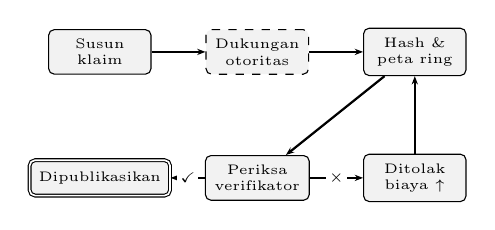
\begin{tikzpicture}[
    stp/.style={draw, rounded corners=2pt, minimum width=1.3cm, minimum height=0.45cm, align=center, font=\tiny, fill=black!5},
    arr/.style={-{Stealth[length=3pt]}, thick},
    lbl/.style={font=\tiny, fill=white, inner sep=1pt}
]
\node[stp] (comp) at (0,0) {Susun\\klaim};
\node[stp, dashed] (auth) at (2.0,0) {Dukungan\\otoritas};
\node[stp] (hash) at (4.0,0) {Hash \&\\peta ring};
\node[stp] (ver) at (2.0,-1.6) {Periksa\\verifikator};
\node[stp, double] (pub) at (0,-1.6) {Dipublikasikan};
\node[stp] (rej) at (4.0,-1.6) {Ditolak\\biaya $\uparrow$};

\draw[arr] (comp) -- (auth);
\draw[arr] (auth) -- (hash);
\draw[arr] (hash) -- (ver);
\draw[arr] (ver) -- node[lbl] {\checkmark} (pub);
\draw[arr] (ver) -- node[lbl] {$\times$} (rej);
\draw[arr] (rej) -- ++(0,0.8) -| (hash);
\end{tikzpicture}
\caption{Siklus hidup klaim dengan lingkaran iterasi.}
\label{fig:lifecycle}
\end{figure}

\subsection{Hubungan dengan W3C DID Core}

Model identitas RSN adalah superset yang tepat dari spesifikasi W3C DID Core~\cite{did2022}. Semua DID RSN adalah DID W3C yang valid. Ekstensi khusus RSN dikodekan sebagai properti dokumen DID yang didefinisikan dalam spesifikasi metode DID khusus, kompatibel dengan infrastruktur yang ada seperti ION~\cite{buchner2021} dan Ceramic~\cite{ceramic2023}.

% ============================================================
% 5. VERIFICATION AND PROPAGATION
% ============================================================
\section{Verifikasi dan Propagasi Informasi}

\subsection{Biaya Pemasukan Informasi}

Prinsip ekonomi inti RSN adalah asimetri antara membaca dan menulis. Membaca data reputasi mendekati biaya marjinal nol bagi peserta yang merupakan bagian dari jaringan DID dan memiliki akses yang sepadan dengan reputasi mereka---pendatang baru harus secara bertahap memperoleh akses yang lebih luas (lihat anti-leeching). Menulis---dipahami sebagai materialisasi reputasi yang tahan lama ke dalam jaringan, bukan sebagai tindakan teknis sekali pakai---memerlukan investasi kumulatif yang dapat diverifikasi di tiga dimensi: \textbf{waktu} (bertahun-tahun kehidupan yang dihabiskan untuk perilaku konsisten, komitmen yang dipenuhi, dan hubungan yang dipupuk), \textbf{energi} (upaya yang diinvestasikan dalam kejujuran, kepedulian terhadap kemitraan, dan keterpercayaan jangka panjang), dan \textbf{uang} (investasi pada nama diri sendiri---pengembangan profesional, kualitas pekerjaan seseorang, restitusi atas kerugian yang ditimbulkan). Reputasi tidak dapat dibeli secara instan---ia adalah hasil dari akumulasi seumur hidup yang hanya dibuat terlihat dan dapat dipindahkan lintas konteks oleh sistem. Biaya teknis sekali pakai dari protokol (tanda tangan kriptografis, biaya verifikator) dapat diabaikan dibandingkan dengan investasi yang mendasarinya ini.

\subsection{Grafik Sosial dan Kedalaman Kontak}

RSN pada dasarnya adalah jaringan sosial: setiap DID menambahkan kontak (DID lain) yang mengizinkan koneksi tersebut. Kontak-kontak ini memiliki kontak mereka sendiri, dan seterusnya. Pencarian verifikator algoritmik beroperasi dalam kedalaman kontak tertaut yang dapat dikonfigurasi $h$ (mis., $h=3$: kontak langsung seseorang, kontak mereka, dan kontak dari kontak). Arsitektur ini tidak memerlukan satu blockchain global tunggal---ia secara alami mendukung munculnya komunitas/klaster dengan tumpang tindih ke komunitas lain. Setiap peserta DID harus memiliki \textbf{kebijakan} yang dipublikasikan---seperangkat aturan yang dapat dibaca mesin yang mengatur bagaimana permintaan masuk dievaluasi. Pelanggaran kebijakan dicatat dalam jaringan sebagai artefak negatif.

\subsection{Pemilihan Verifikator Algoritmik}

Protokol verifikasi menggunakan consistent hashing~\cite{karger1997} (Gbr.~\ref{fig:verifier}). Verifikasi adalah layanan berbayar: verifikator beroperasi dengan imbalan, menciptakan pasar di mana persaingan mendorong penetapan harga, kecepatan, dan keandalan.

\textbf{Langkah 1.} Dokumen klaim digabungkan dengan hasil hash iterasi sebelumnya (atau $\varnothing$ pada iterasi pertama) dan di-hash:
\begin{equation}
\text{pos} = f_h(\text{claim} \| \text{prev\_hash})
\label{eq:hash}
\end{equation}

Algoritma harus menyertakan \emph{jalur lengkap} dari semua permintaan dan respons sebelumnya---bukan sekadar hash dari iterasi sebelumnya. Respons penuh setiap verifikator (penerimaan, penolakan, harga yang dikutip, alasan) ditambahkan ke dokumen yang terus bertambah, dapat diverifikasi melalui tanda tangan kriptografis pada setiap langkah.

\textbf{Langkah 2.} Hash dipetakan ke $N$ posisi pada consistent hash ring, terdistribusi secara merata (mis., untuk $N=4$: $+0^{\circ}, +90^{\circ}, +180^{\circ}, +270^{\circ}$). Dari setiap posisi, pencarian searah jarum jam memilih DID terdekat sebagai kandidat verifikator (Gbr.~\ref{fig:multipoint}). $N$ adalah parameter variabel yang dapat bergantung pada persentase DID yang sedang aktif, waktu dalam sehari, atau responsivitas jaringan historis.

\textbf{Langkah 3.} Verifikator menerima (memublikasikan, mempertaruhkan reputasi) atau menolak (kembali ke Langkah~1 dengan hash penolakan). Ketika sebuah node tidak merespons meskipun menyatakan status online, permintaan berikutnya harus menyertakan semua respons dari seluruh $N$ kandidat verifikator sebelumnya.

\textbf{Anti-leeching.} DID target dapat menetapkan biaya atau pembatasan akses untuk kueri dari DID baru dengan reputasi kecil. Mekanisme berjenjang ini (bukan biner) memaksa pendatang baru untuk membangun reputasi melalui aktivitas yang tulus sebelum secara bebas mengonsumsi data orang lain.

\begin{figure}[ht]
\centering
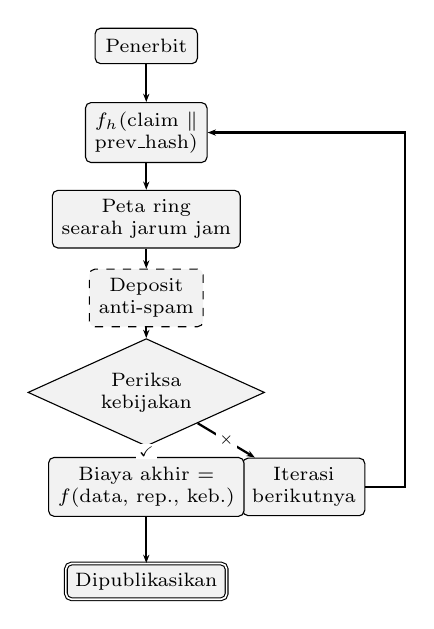
\begin{tikzpicture}[
    box/.style={draw, rounded corners=2pt, minimum width=1.3cm, minimum height=0.45cm, align=center, font=\scriptsize, fill=black!5},
    dec/.style={draw, diamond, aspect=2.2, minimum width=0.9cm, align=center, font=\scriptsize, fill=black!5},
    arr/.style={-{Stealth[length=3pt]}, thick},
    lbl/.style={font=\tiny, fill=white, inner sep=1pt}
]
\node[box] (iss) at (0,0) {Penerbit};
\node[box] (hash) at (0,-1.1) {$f_h$(claim $\|$\\prev\_hash)};
\node[box] (ring) at (0,-2.2) {Peta ring\\searah jarum jam};
\node[box, dashed] (spam) at (0,-3.2) {Deposit\\anti-spam};
\node[dec] (check) at (0,-4.4) {Periksa\\kebijakan};
\node[box] (rej) at (2,-5.6) {Iterasi\\berikutnya};
\node[box] (fee) at (0,-5.6) {Biaya akhir =\\$f$(data, rep., keb.)};
\node[box, double] (pub) at (0,-6.8) {Dipublikasikan};

\draw[arr] (iss) -- (hash);
\draw[arr] (hash) -- (ring);
\draw[arr] (ring) -- (spam);
\draw[arr] (spam) -- (check);
\draw[arr] (check) -- node[lbl] {$\times$} (rej);
\draw[arr] (check) -- node[lbl] {\checkmark} (fee);
\draw[arr] (fee) -- (pub);
\draw[arr] (rej.east) -- ++(0.5,0) |- (hash.east);
\end{tikzpicture}
\caption{Protokol pemilihan verifikator. Deposit anti-spam bersifat opsional dan dapat dikembalikan. Biaya akhir dibayar hanya pada saat penerimaan.}
\label{fig:verifier}
\end{figure}

Setiap penolakan menambahkan respons penuh verifikator (termasuk alasan dan kondisi) ke dokumen klaim, memperluas isinya. Dari dokumen yang diperluas tersebut, sebuah hash baru dihitung secara nondeterministik, dipetakan ke posisi ring yang berbeda dan memilih verifikator yang berbeda. Dokumentasi jalur lengkap bersifat wajib---penerbit tidak dapat memprediksi atau memengaruhi verifikator berikutnya. Jika seorang verifikator mengabaikan permintaan meskipun kebijakan yang dinyatakan kompatibel, para saksi (jika hadir) mencatat hal ini, dan penerbit dapat melampirkan bukti saksi saat publikasi akhir.

\begin{figure}[ht]
\centering
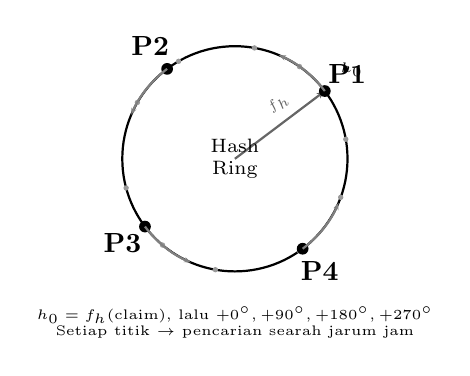
\begin{tikzpicture}[scale=0.65]
% Ring
\draw[thick] (0,0) circle (2.2cm);
% DID nodes on ring
\foreach \a in {10,55,80,120,150,195,230,260,305,340} {
  \fill[black!40] (\a:2.2) circle (1.5pt);
}
% Hash offset arrow pointing to initial position
\draw[-{Stealth[length=3pt]}, thick, black!60] (0,0) -- node[font=\tiny,above,sloped,pos=0.6] {$f_h$} (37:2.2);
\fill[black] (37:2.2) circle (2pt);
\node[font=\tiny,anchor=south west] at (37:2.35) {$h_0$};
% N=4 points offset from h0 by +0, +90, +180, +270
\foreach \offset/\l in {0/P1,90/P2,180/P3,270/P4} {
  \pgfmathsetmacro{\ang}{37+\offset}
  \node[fill=black, circle, inner sep=1.5pt] (p\offset) at (\ang:2.2) {};
  \node[font=\tiny,font=\bfseries] at (\ang:2.75) {\l};
  % clockwise search arc
  \draw[-{Stealth[length=2.5pt]}, thick, gray] (\ang:2.2) arc (\ang:\ang+30:2.2);
}
\node[font=\scriptsize, align=center] at (0,0) {Hash\\Ring};
\node[font=\tiny, align=center] at (0,-3.2) {$h_0 = f_h(\text{claim})$, lalu $+0^{\circ},+90^{\circ},+180^{\circ},+270^{\circ}$\\Setiap titik $\rightarrow$ pencarian searah jarum jam};
\end{tikzpicture}
\caption{Pemilihan multi-titik ($N{=}4$). Hash $h_0$ menetapkan offset; 4 titik terdistribusi merata dari $h_0$.}
\label{fig:multipoint}
\end{figure}

\subsection{Protokol Saksi}

Peran \textbf{Saksi} menyediakan akuntabilitas inkognito untuk kejujuran verifikator melalui protokol kode-tantangan kriptografis:

\textbf{Langkah W1.} Peminta menandatangani permintaan verifikasi dan mengirimkannya kepada $N_w$ saksi---kontak dari jaringan sosial peminta, atau penyedia layanan saksi khusus yang beroperasi dengan imbalan.

\textbf{Langkah W2.} Setiap saksi $w_i$ menandatangani seluruh permintaan yang telah ditandatangani, menyimpan tanda tangan asli $\sigma_i$, dan menghitung kode tantangan $c_i = h(\sigma_i)$. Kode tantangan tersebut ditambahkan ke permintaan.

\textbf{Langkah W3.} Permintaan tersebut, yang kini membawa $N_w$ kode tantangan, dikirim ke verifikator. Verifikator mengamati kode-kode tersebut tetapi \emph{tidak dapat menentukan} siapa para saksinya atau apakah kode-kode tersebut sesuai dengan tanda tangan yang nyata.

\textbf{Langkah W4 (verifikator jujur).} Jika verifikator merespons sesuai dengan kebijakan yang dinyatakannya, kode tantangan tetap tidak transparan. Saksi tidak pernah terungkap. Tidak ada data tambahan yang dipublikasikan.

\textbf{Langkah W5 (pelanggaran kebijakan).} Jika verifikator melanggar kebijakannya (mengabaikan permintaan, merespons secara tidak konsisten), peminta memegang tanda tangan asli para saksi $\sigma_i$. Tanda tangan ini dapat dipublikasikan sebagai data pendamping: siapa pun dapat memverifikasi $c_i = h(\sigma_i)$, membuktikan bahwa saksi tersebut hadir. Peminta dapat memublikasikan secara independen---verifikator sudah menandatangani kode tantangan dalam responsnya.

\textbf{Sifat gertakan.} Peminta dapat mengganti sebagian atau seluruh kode tantangan dengan nilai acak. Verifikator tidak dapat membedakan kode asli (didukung oleh otoritas bereputasi tinggi) dari noise. \emph{Ketidakpastian} ini adalah mekanisme penegakannya: setiap permintaan membawa risiko bahwa suatu otoritas yang dihormati sedang mengawasi secara inkognito. Biaya untuk mempertahankan tekanan ini nyaris nol (menghasilkan angka acak), sementara potensi biaya ketidakjujuran bagi verifikator bersifat katastrofik. Perilaku jujur pun terinsentifkan bahkan tanpa kehadiran saksi yang sebenarnya.

\textbf{Otoritas sebagai saksi.} Sebuah Otoritas yang mendukung suatu klaim dapat menggabungkan layanan saksi: ``Saya mendukung klaim Anda dan bertindak sebagai saksi inkognito selama verifikasi.'' Ini adalah model bisnis yang alami---Otoritas sudah memiliki konteksnya. Namun, kedua peran tersebut secara logis independen.

\subsection{Prinsip Radikalisme yang Mahal}

Tiga saluran biaya bergabung secara bersamaan (Gbr.~\ref{fig:radicalism}):

\textbf{Saluran 1: Biaya Iterasi.} Setiap penolakan memaksa iterasi baru yang memakan waktu dan sumber daya. Pertumbuhan linear.

\textbf{Saluran 2: Pembengkakan Dokumen.} Setiap iterasi menambahkan respons penuh verifikator ke dokumen klaim. Pertumbuhannya linear, tetapi dengan offset dasar: muatan awal (isi klaim, dukungan otoritas, tanda tangan kriptografis) sudah memiliki ukuran yang tidak sepele $B_0$. Ukuran total setelah $k$ iterasi: $S(k) = B_0 + k \cdot \Delta$, di mana $\Delta$ adalah ukuran respons rata-rata.

\textbf{Saluran 3: Premi Risiko Verifikator.} Risiko bersifat subjektif. Verifikator menilai apakah kebijakan yang dinyatakan DID peminta bertentangan dengan kepentingan komersial, sosial, atau politik verifikator itu sendiri. Premi tersebut dapat meningkat secara eksponensial seiring persepsi jarak dari ``ideal'' verifikator: $P(d) = \alpha \cdot e^{\beta d}$, di mana $d$ adalah metrik jarak subjektif verifikator. Melampaui batas larangan pribadi, verifikator dapat menolak sepenuhnya.

\begin{figure}[ht]
\centering
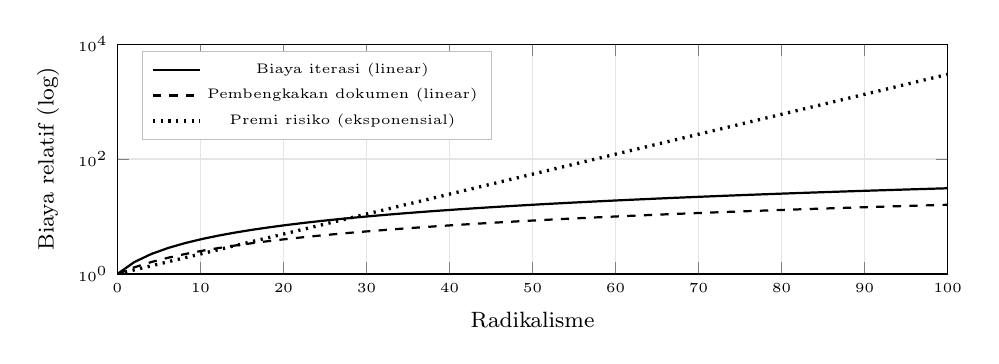
\begin{tikzpicture}
\begin{axis}[
    width=\columnwidth,
    height=4.5cm,
    xlabel={\footnotesize Radikalisme},
    ylabel={\footnotesize Biaya relatif (log)},
    ymode=log,
    xmin=0, xmax=100,
    ymin=1, ymax=10000,
    grid=major,
    grid style={gray!20},
    legend style={at={(0.03,0.97)},anchor=north west,font=\tiny,draw=gray!50},
    tick label style={font=\tiny},
    label style={font=\footnotesize},
]
\addplot[black, thick, domain=0:100, samples=50] {1 + 0.3*x};
\addlegendentry{Biaya iterasi (linear)}
\addplot[black, thick, dashed, domain=0:100, samples=50] {1 + 0.15*x};
\addlegendentry{Pembengkakan dokumen (linear)}
\addplot[black, thick, dotted, line width=1.2pt, domain=0:100, samples=100] {exp(0.08*x)};
\addlegendentry{Premi risiko (eksponensial)}
\end{axis}
\end{tikzpicture}
\caption{Eskalasi biaya di tiga saluran. Premi risiko mendominasi pada radikalisme tinggi.}
\label{fig:radicalism}
\end{figure}

Yang krusial, ini bukan sensor. Tidak ada klaim yang dilarang. Sistem menetapkan harga risiko (Tabel~\ref{tab:costs}).

\begin{table}[ht]
\centering
\caption{Perbandingan biaya di berbagai jenis klaim.}
\label{tab:costs}
\footnotesize
\begin{tabular}{@{}lcccc@{}}
\toprule
\textbf{Jenis} & \textbf{Iter.} & \textbf{Dok} & \textbf{Biaya} & \textbf{Total} \\
\midrule
Kredibel & $k_{\min}$ & $B_0$ & $P_{\min}$ & Rendah \\
Kontroversial & $k_{\text{med}}$ & $B_0{+}k\Delta$ & $\alpha e^{\beta d}$ & Sedang \\
Radikal & $k_{\max}$ & $\gg B_0$ & $\gg P_{\min}$ & Sangat tinggi \\
Curang & $\to\infty$ & --- & --- & Tak dapat dipublikasikan \\
\bottomrule
\end{tabular}
\end{table}

% ============================================================
% 6. REPUTATION AND RISK
% ============================================================
\section{Reputasi dan Penilaian Risiko}

\subsection{Model Akumulasi Reputasi}

Reputasi menunjukkan tiga sifat: \textbf{akumulasi lambat} (pertumbuhan bertahap melalui perilaku konsisten), \textbf{penghancuran cepat} (satu kecurangan dapat menurunkan skor secara katastrofik), dan \textbf{evaluasi individual} (setiap pihak yang mengonsumsi dapat menerapkan fungsi agregasinya sendiri).

\subsection{Otoritas Bereputasi}

Sebuah Otoritas Bereputasi meninjau klaim dan, jika puas, ikut menandatanganinya---mempertaruhkan reputasinya sendiri (Gbr.~\ref{fig:authority}). Asimetri ini disengaja: memperoleh reputasi berjalan lambat (bertahap $+\delta$ per dukungan yang jujur), sementara kehilangannya bersifat katastrofik ($-\Delta \gg \delta$ per dukungan palsu; sebagai ilustrasi, mis., $+2\%$ vs.\ $-70\%$). Strategi optimalnya selalu menolak klaim yang mencurigakan. Nilai spesifik $\delta$ dan $\Delta$ merupakan parameter sistem.

\begin{figure}[ht]
\centering
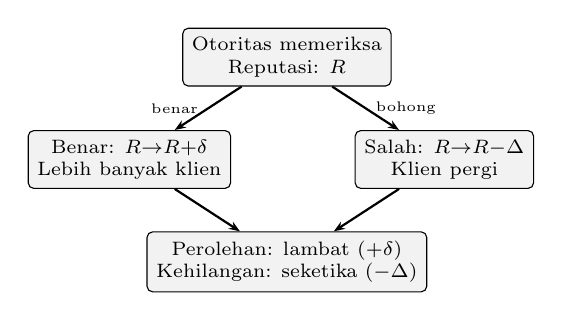
\begin{tikzpicture}[
    box/.style={draw, rounded corners=2pt, minimum width=2cm, minimum height=0.6cm, align=center, font=\scriptsize, fill=black!5},
    arr/.style={-{Stealth[length=4pt]}, thick}
]
\node[box] (exam) at (0,0) {Otoritas memeriksa\\Reputasi: $R$};
\node[box] (true) at (-2,-1.3) {Benar: $R{\to}R{+}\delta$\\Lebih banyak klien};
\node[box] (false) at (2,-1.3) {Salah: $R{\to}R{-}\Delta$\\Klien pergi};
\node[box] (insight) at (0,-2.6) {Perolehan: lambat ($+\delta$)\\Kehilangan: seketika ($-\Delta$)};

\draw[arr] (exam) -- node[left,font=\tiny] {benar} (true);
\draw[arr] (exam) -- node[right,font=\tiny] {bohong} (false);
\draw[arr] (true) -- (insight);
\draw[arr] (false) -- (insight);
\end{tikzpicture}
\caption{Otoritas Bereputasi---insentif asimetris.}
\label{fig:authority}
\end{figure}

\subsection{Reputasi Multidimensi}

Reputasi bukanlah skalar melainkan vektor di berbagai dimensi: keandalan finansial, integritas pribadi, kompetensi profesional, keterlibatan sipil, dan lainnya (Gbr.~\ref{fig:reputation-radar}). Penyedia evaluasi yang berbeda memproyeksikan vektor ini secara berbeda tergantung konteks---pemberi pinjaman memprioritaskan keandalan finansial, pemberi kerja kompetensi profesional, tetangga perilaku sipil. Tidak ada satu skor reputasi yang ``benar'' tunggal; hanya perspektif.

\begin{figure}[ht]
\centering
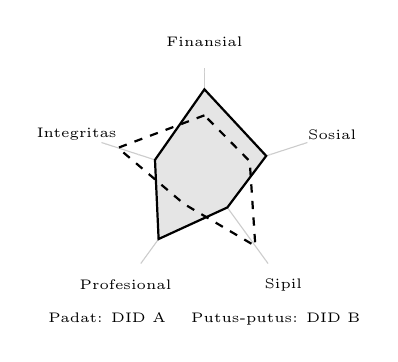
\begin{tikzpicture}[scale=0.55]
\foreach \a/\l in {90/Finansial,162/Integritas,234/Profesional,306/Sipil,18/Sosial} {
  \draw[gray!40] (0,0) -- (\a:2.5);
  \node[font=\tiny, align=center] at (\a:3.1) {\l};
  \foreach \r in {0.8,1.6,2.4} {
    \fill[black!15] (\a:\r) circle (0.5pt);
  }
}
\draw[thick, fill=black!10] (90:2.0) -- (162:1.2) -- (234:1.8) -- (306:0.9) -- (18:1.5) -- cycle;
\draw[thick, dashed] (90:1.4) -- (162:2.1) -- (234:0.8) -- (306:2.0) -- (18:1.1) -- cycle;
\node[font=\tiny] at (0,-3.3) {Padat: DID A \quad Putus-putus: DID B};
\end{tikzpicture}
\caption{Vektor reputasi multidimensi. DID yang berbeda menunjukkan profil yang berbeda di berbagai dimensi.}
\label{fig:reputation-radar}
\end{figure}

\subsection{Penilaian Risiko yang Terdemokratisasi}

RSN mendemokratisasi penilaian risiko sistematis---sebuah kapabilitas yang saat ini terkonsentrasi pada institusi keuangan tetapi dapat diterapkan jauh melampaui perbankan. Konglomerat industri yang menilai keandalan pemasok, perusahaan asuransi yang menetapkan harga risiko perilaku, uji tuntas untuk merger dan akuisisi, estimasi masa pakai peralatan dalam manufaktur---di mana pun risiko pihak lawan memerlukan penilaian, RSN menyediakan alternatif yang terdesentralisasi dan berbasis pasar. Sebuah pasar layanan interpretasi menerjemahkan data reputasi multidimensi mentah menjadi ringkasan yang dapat ditindaklanjuti, membuat evaluasi pihak lawan dapat diakses oleh peserta mana pun dengan biaya marjinal.

% ============================================================
% 7. CONSENSUS AND DISPUTE RESOLUTION
% ============================================================
\section{Konsensus dan Penyelesaian Sengketa}

\subsection{Model Keadilan Terdesentralisasi}

RSN membingkai ulang keadilan sebagai masalah negosiasi bilateral. Ancaman kerusakan reputasi yang permanen dan dapat diverifikasi merupakan pencegah yang lebih efektif daripada proses hukum yang tidak mampu ditanggung oleh pihak yang dirugikan.

\subsection{Konsensus Emergen}

Setiap peserta mempertahankan ambang batas kepuasan pribadi. Konsensus agregat jaringan muncul sebagai rata-rata statistik dari ribuan negosiasi bilateral (Gbr.~\ref{fig:consensus}). Respons yang jauh di atas konsensus (barbar) mahal untuk dipublikasikan. Respons yang dekat dengan konsensus (proporsional) murah. Konsensus bukanlah sebuah aturan---ia adalah sinyal harga.

\begin{figure}[ht]
\centering
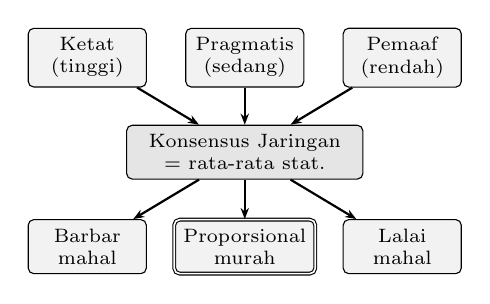
\begin{tikzpicture}[
    person/.style={draw, rounded corners=2pt, minimum width=1.5cm, minimum height=0.5cm, align=center, font=\scriptsize, fill=black!5},
    arr/.style={-{Stealth[length=4pt]}, thick}
]
\node[person] (a) at (-2,0) {Ketat\\(tinggi)};
\node[person] (b) at (0,0) {Pragmatis\\(sedang)};
\node[person] (c) at (2,0) {Pemaaf\\(rendah)};
\node[person, fill=black!10, minimum width=3cm] (cons) at (0,-1.2) {Konsensus Jaringan\\= rata-rata stat.};
\node[person] (exp) at (-2,-2.4) {Barbar\\mahal};
\node[person, double] (prop) at (0,-2.4) {Proporsional\\murah};
\node[person] (neg) at (2,-2.4) {Lalai\\mahal};

\draw[arr] (a) -- (cons);
\draw[arr] (b) -- (cons);
\draw[arr] (c) -- (cons);
\draw[arr] (cons) -- (exp);
\draw[arr] (cons) -- (prop);
\draw[arr] (cons) -- (neg);
\end{tikzpicture}
\caption{Konsensus emergen dari ambang batas kepuasan individual.}
\label{fig:consensus}
\end{figure}

\subsection{Kalibrasi Hukuman}

Setiap Pemegang DID secara publik menyatakan respons terhadap kategori pelanggaran tertentu. Pernyataan yang terlalu keras atau terlalu lunak secara tidak proporsional menarik sinyal reputasi negatif. Pernyataan yang proporsional diterima tanpa gesekan---sebuah sistem hukuman yang mengalibrasi diri sendiri.

Pernyataan konsensus itu sendiri tunduk pada deteksi kemunafikan: berkomitmen secara deklaratif pada posisi konsensus sambil berperilaku secara tidak konsisten merupakan pelanggaran reputasi yang lebih berat daripada penyimpangan yang mendasarinya, karena hal itu menunjukkan penipuan yang disengaja.

\subsection{Pendelegasian}

Semua aktivitas dalam sebuah DID---dengan satu pengecualian---dapat didelegasikan ke DID lain. \textbf{Peran Subjek---DID yang perilakunya menjadi objek klaim---tidak dapat didelegasikan; ia terikat secara tidak dapat dipindahtangankan kepada pemegang identitas yang dirujuk oleh klaim tersebut.} Peran aktif lainnya---Penerbit, Otoritas, Saksi, Verifikator---dapat dipindahkan ke DID delegasi yang ditunjuk, baik untuk verifikasi, pengajuan klaim, partisipasi konsensus, maupun penyelesaian sengketa. Pendelegasian dapat dicabut kapan saja. Ini memungkinkan spesialisasi (mis., layanan verifikasi profesional) sementara Pemegang mempertahankan kendali dan tanggung jawab tertinggi. Pendelegasian berlaku di seluruh sistem dan sangat penting untuk skalabilitas.

\subsection{Dari Moralitas Individu ke Kontrak Sosial Emergen}

Kebijakan yang dinyatakan setiap DID merepresentasikan formalisasi moralitas individu: apa yang dianggap dapat diterima oleh Pemegang, bagaimana mereka merespons perilaku tertentu, apa yang mereka syaratkan dari pihak lawan. Kebijakan-kebijakan ini tidak dipaksakan oleh perancang sistem---ia dipilih oleh setiap peserta dan diekspresikan dalam bentuk yang dapat dibaca mesin.

Formalisasi ini memungkinkan kemunculan tiga tahap. Pertama, moralitas individu dikodekan sebagai \textbf{kebijakan}---seperangkat aturan, ambang batas, dan fungsi respons yang dinyatakan yang dijanjikan DID untuk diikuti. Kedua, agregat dari semua kebijakan di seluruh jaringan menghasilkan \textbf{etika emergen}---norma-norma yang dapat diamati secara statistik yang tidak dirancang oleh satu peserta pun tetapi muncul dari interaksi ribuan posisi moral individu~\cite{durkheim1893}. Ketiga, etika emergen ini, yang diekspresikan sebagai norma perilaku bersama yang ditegakkan melalui sinyal harga bilateral, membentuk sebuah \textbf{kontrak sosial yang terukur}---bukan konstruksi teoretis yang tak seorang pun menandatanganinya~\cite{rawls1971}, melainkan seperangkat aturan yang dapat diamati secara empiris dan didukung oleh perilaku nyata.

Proses ini mencerminkan temuan dari teori moral foundations~\cite{haidt2012}: moralitas manusia bersifat intuitif, pluralistik, dan bervariasi secara budaya. RSN tidak memerlukan konsensus moral sebagai input; ia menghasilkan konsensus perilaku sebagai output. Kontrak sosial yang dihasilkan tidaklah statis---ia berkembang seiring peserta bergabung, keluar, dan menyesuaikan kebijakan mereka sebagai respons terhadap umpan balik jaringan. Berbeda dengan teori kontrak sosial klasik, kontrak ini dapat dicabut, dapat diamati, dan dapat ditegakkan tanpa seorang penguasa berdaulat.

% ============================================================
% 8. ECONOMIC MODEL
% ============================================================
\section{Model Ekonomi}

Bagian-bagian sebelumnya menjelaskan sebuah alat---mekanisme verifikasi RSN, struktur biaya, dan konsensus emergen. Bagian ini menjelaskan sebuah metodologi untuk menerapkan alat ini pada transisi fiskal dan tata kelola. Alatnya bersifat serbaguna; metodologi di bawah ini adalah satu aplikasi yang mungkin.

\subsection{Struktur Insentif}

Reputasi sebagai modal menciptakan insentif langsung untuk perilaku jujur. Dalam operasi normal, peserta membangun reputasi secara alami melalui transaksi sehari-hari dan komitmen yang dipenuhi. Pengeluaran utama adalah untuk klaim \emph{negatif}---mencatat kerugian yang ditimbulkan oleh orang lain. Asimetri ini menginsentifkan perilaku yang berguna dan andal: bersikap jujur tidak menimbulkan biaya tambahan, sementara bersikap merugikan menciptakan jejak terdokumentasi yang akan dibayar orang lain untuk dipertahankan. Kemunafikan---menyatakan aturan tanpa mengikutinya---adalah mode kegagalan yang paling mahal, karena hal itu menunjukkan penipuan yang disengaja.

\subsection{Sistem Fiskal Paralel}

Tiga komponen memungkinkan tekanan kompetitif: (1)~\textbf{Pajak Sederhana}---satu tarif proporsional tunggal tanpa pengecualian, awalnya sedikit di bawah tarif efektif yang berlaku; (2)~\textbf{Registrasi Pengeluaran Elektronik (ESR)}---membalik model EET Ceko sehingga warga negara mengawasi pengeluaran negara; (3)~\textbf{Alokasi Pajak yang Diarahkan Warga}---dimulai dari beberapa persen pada tahun pertama dan mencapai, setelah satu dekade, di mana pun dari puluhan rendah hingga migrasi penuh ke sistem yang diarahkan warga, tergantung pada laju adopsi. Tempo aktualnya bergantung pada kecepatan munculnya alternatif pasar bebas terhadap layanan negara dan pada kesediaan negara untuk bekerja sama dengan transisi tersebut; fungsi waktu tidak harus linear, dan tidak ada alasan untuk menetapkan batas atas mengenai di mana adopsi pada akhirnya dapat tiba.

% ============================================================
% 9. MIGRATION PATH
% ============================================================
\section{Jalur Migrasi}

Migrasi berlangsung melalui tiga fase (Gbr.~\ref{fig:migration}): \textbf{Fase~1: Overlay} (RSN sebagai lapisan informasional, negara adalah satu-satunya penyedia), \textbf{Fase~2: Persaingan} (RSN menyediakan alternatif fungsional, penggunaan sistem ganda), dan \textbf{Fase~3: Transisi} (RSN mengungguli padanan negara, migrasi sukarela). Transisi ini dapat dibalik pada setiap tahap.

\begin{figure}[ht]
\centering
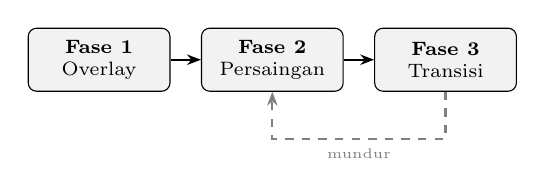
\begin{tikzpicture}[
    phase/.style={draw, rounded corners=3pt, minimum width=1.8cm, minimum height=0.8cm, align=center, font=\scriptsize, fill=black!5},
    arr/.style={-{Stealth[length=5pt]}, thick}
]
\node[phase] (p1) at (0,0) {\textbf{Fase 1}\\Overlay};
\node[phase] (p2) at (2.2,0) {\textbf{Fase 2}\\Persaingan};
\node[phase] (p3) at (4.4,0) {\textbf{Fase 3}\\Transisi};

\draw[arr] (p1) -- (p2);
\draw[arr] (p2) -- (p3);
\draw[arr, dashed, gray] (p3.south) -- ++(0,-0.6) -| node[below,font=\tiny,pos=0.25] {mundur} (p2.south);
\end{tikzpicture}
\caption{Migrasi tiga fase---dapat dibalik pada setiap tahap.}
\label{fig:migration}
\end{figure}

Mekanisme tekanan utama bersifat fiskal: ketika para pembayar pajak bersyarat mencapai ``minoritas yang signifikan secara ekonomi $X$''---sebuah kelompok yang cukup besar sehingga penindasan terhadapnya menyebabkan kerusakan ekonomi yang tidak sepele dan pembangkangan sipil menjadi ancaman yang kredibel---negara pun memasuki negosiasi. Untuk ilustrasi, kami menggunakan $X \approx 15\%$ dari PDB, tetapi ambang batas aktualnya bergantung pada ekonomi yang spesifik.

% ============================================================
% 10. SECURITY ANALYSIS
% ============================================================
\section{Analisis Keamanan}

Kami mempertimbangkan lima kategori musuh: pelaku jahat individu, kelompok terorganisir, musuh korporat, musuh tingkat negara, dan musuh tingkat protokol.

\textbf{Ketahanan Sybil}~\cite{douceur2002}. Membangun reputasi memerlukan interaksi yang berkelanjutan dan dapat diverifikasi. Biaya serangan Sybil yang berhasil berskala linear dengan jumlah identitas palsu dan kuadratik dengan tingkat reputasi target. Mengoperasikan beberapa DID secara paralel dimungkinkan tetapi mahal secara desain---setiap identitas harus mengakumulasikan reputasi secara independen melalui aktivitas yang tulus. Dalam masyarakat bebas biaya ini mencegah penyalahgunaan sembarangan; dalam kediktatoran, DID paralel menjadi alat bertahan hidup yang memungkinkan perlawanan terkompartementalisasi, koordinasi bawah tanah, dan navigasi pasar gelap yang lebih aman.

\textbf{Pertahanan terhadap kolusi.} Pola dukungan timbal balik di antara kelompok tertutup dapat dideteksi melalui analisis grafik sosial. Fungsi agregasi reputasi mendiskon klaim dari sumber yang berkerumun secara rapat.

\textbf{Musuh tingkat negara.} Onion routing, ketiadaan infrastruktur tersentralisasi, dan distribusi peran Verifikator ke seluruh basis peserta memastikan bahwa penindasan memerlukan tindakan yang tidak sebanding dengan manfaat apa pun.

\textbf{Privasi vs.\ akuntabilitas.} Pseudonimitas---jalan tengah antara anonimitas dan pengungkapan identitas---memungkinkan DID untuk mengakumulasikan reputasi yang bermakna tanpa mengungkapkan identitas dunia nyata Pemegang.

% ============================================================
% 11. PRIVACY
% ============================================================
\section{Pertimbangan Privasi}

Model privasi RSN dibangun di atas pseudonimitas. Pemegang mengendalikan pengungkapan identitas: minimal (pseudonim murni), selektif (kredensial tertentu ditautkan), atau penuh (identitas hukum terkait). Klaim yang dipublikasikan bersifat permanen---sistem mendukung koreksi kontekstual tetapi bukan penghapusan. Seorang Pemegang dapat meninggalkan DID yang telah dikompromikan dan memulai kembali, dengan merelakan reputasi yang telah diakumulasikan.

% ============================================================
% 12. RELATED WORK
% ============================================================
\section{Karya Terkait}

Spesifikasi W3C DID Core~\cite{did2022} dan Ceramic Network~\cite{ceramic2023} menyediakan fondasi identitas. EigenTrust~\cite{kamvar2003} mendemonstrasikan agregasi reputasi terdistribusi tanpa otoritas pusat. SBT~\cite{weyl2022} memperkenalkan token sosial yang tidak dapat dipindahtangankan. RSN berbeda dalam penekanannya pada biaya ekonomi sebagai filter kualitas dan mekanismenya untuk menetapkan harga radikalisme.

DAO~\cite{buterin2014} dan quadratic voting~\cite{buterin2019} mendemonstrasikan kelayakan tata kelola terdesentralisasi. RSN menurunkan konsensus dari negosiasi harga bilateral alih-alih pemungutan suara.

Proposal ini menarik dari teori anarko-kapitalis~\cite{rothbard1973,hoppe2001} untuk penyediaan layanan swasta tetapi menyimpang dalam dua hal kritis: ia merancang untuk kedengkian dan dorongan pembalasan alih-alih mengasumsikan rasionalitas, dan ia mengusulkan transisi bertahap alih-alih revolusi. Konsep kontrak sosial emergen memiliki pendahulu dalam teori tatanan spontan Hayek~\cite{hayek1973}.

\textbf{Anarko-agorisme.} RSN memiliki banyak kesamaan dengan counter-economics agoris~\cite{konkin2006}---terutama penekanan pada membangun institusi paralel dan pertukaran sukarela. Namun, agorisme cenderung mengasumsikan kepentingan-diri yang rasional sebagai mekanisme koordinasi yang memadai dan seringkali tidak memiliki jalur migrasi konkret dari struktur negara yang ada. RSN secara eksplisit menyertakan kecenderungan perilaku non-rasional dan menyediakan mekanisme tekanan fiskal untuk transisi bertahap.

\textbf{Meritokrasi.} RSN mungkin merepresentasikan deskripsi fungsional pertama tentang bagaimana meritokrasi~\cite{young1958} dapat muncul sebagai properti sistemik alih-alih sekadar slogan. Sistem meritokratik tradisional gagal karena mereka memerlukan otoritas pusat untuk mendefinisikan dan menegakkan ``jasa''. Dalam RSN, jasa muncul dari evaluasi bilateral: mereka yang memberikan nilai mengakumulasikan reputasi; tidak ada komite yang memutuskan siapa yang memiliki jasa.

\textbf{Properti sebagai privilese.} RSN menyimpang secara fundamental dari perlakuan anarko-kapitalis dan mazhab Austria terhadap hak milik sebagai sesuatu yang alami dan absolut. Dalam kerangka RSN, properti adalah sebuah \emph{privilese}---pengakuan sosial yang, dalam kasus ekstrem, dapat ditarik oleh komunitas ketika seorang peserta secara fundamental melanggar norma bersama (pengkhianatan, penolakan untuk membela komunitas dalam krisis eksistensial, eksploitasi sistematis). Ini bukanlah pengambilalihan oleh negara melainkan penarikan pengakuan sosial oleh jaringan hubungan bilateral.

% ============================================================
% 13. LIMITATIONS
% ============================================================
\section{Diskusi dan Keterbatasan}

\textbf{Cold start.} Nilai RSN bergantung pada efek jaringan; pengadopsi awal menghadapi nilai yang terbatas sampai partisipasi mencapai ambang batas. Namun, bahkan dari tahap awal, jaringan DID berfungsi sebagai sumber informasi pelengkap yang berguna. Evaluasi reputasi awal dan penilaian otoritas diharapkan berkembang secara bertahap dengan kecanggihan yang meningkat.

\textbf{Anti-leeching dan kontrol akses.} DID target dapat menerapkan biaya berjenjang dan pembatasan akses pada kueri dari DID bereputasi rendah. Ini bukan biner melainkan skala kontinu: semakin sedikit reputasi yang dimiliki suatu DID peminta, semakin sedikit informasi yang diterimanya, semakin lama ia menunggu, dan semakin banyak yang harus dibayarnya. Mekanisme ini menginsentifkan partisipasi yang tulus alih-alih konsumsi pasif.

\textbf{Ketimpangan akses.} Biaya memublikasikan klaim dapat menyaring keluhan yang sah dari peserta yang kurang beruntung secara ekonomi. Mitigasi: setiap peserta secara bersamaan berperan sebagai verifikator potensial (atau mendelegasikan peran ini) dan memperoleh biaya verifikasi. Selama horizon waktu yang cukup, seorang peserta non-radikal seharusnya mendekati netralitas finansial---pendapatan verifikasi kurang lebih mengimbangi biaya publikasi. Ini adalah ekspektasi statistik, bukan jaminan.

\textbf{Ketimpangan reputasi.} Pengadopsi awal mengakumulasikan keunggulan yang dapat menciptakan hambatan bagi pendatang belakangan. Namun, evaluasi reputasi dilakukan oleh penyedia pihak ketiga yang dapat memilih untuk memitigasi keunggulan penggerak pertama melalui algoritma agregasi mereka. Menjadi yang pertama dengan reputasi baik adalah keunggulan ekonomi komparatif yang sah---dan itu memang disengaja.

\textbf{Pertanyaan terbuka.} Fungsi biaya optimal, standar agregasi, tata kelola protokol, dan interaksi dengan data reputasi sintetis yang dihasilkan AI tetap menjadi area untuk pekerjaan di masa depan.

Makalah ini tidak mengklaim bahwa RSN akan menghasilkan hasil yang optimal dalam segala keadaan. Ia mengklaim bahwa RSN merepresentasikan sebuah alternatif yang \emph{layak}---dapat diimplementasikan secara teknis, dapat menopang diri sendiri secara ekonomi, dan kompatibel secara sosial dengan kecenderungan perilaku manusia sebagaimana adanya.

% ============================================================
% 14. CONCLUSION
% ============================================================
\section{Kesimpulan}

Makalah ini telah menyajikan Reputation Social Network, sebuah protokol terdesentralisasi yang memungkinkan pertukaran reputasi yang pseudonim dan dapat diverifikasi. Prinsip Radikalisme yang Mahal memastikan bahwa klaim yang curang tersingkir melalui harga tanpa sensor. Jalur migrasi yang diusulkan memungkinkan transisi yang bertahap dan dapat dibalik dari institusi yang ada. Desain ini menyertakan sifat manusia sebagaimana adanya---termasuk kepicikan, kedengkian, dan keinginan akan kepuasan pembalasan---alih-alih menuntut transformasi ideologis. Hasilnya bukanlah utopia melainkan sebuah sistem di mana keadilan dapat diakses, reputasi diperoleh, dan biaya pelanggaran ditanggung oleh pihak yang menyebabkannya.

% ============================================================
% REFERENCES
% ============================================================
\bibliography{references}

\end{document}
